\subsection{Experiment 7A: finite local data and the value of pooling}
\label{sec:experiment7a}

\paragraph{Question.}
The oracle results establish that persistent LPV families can be useful.
Experiment 7A asks whether the available local evidence is insufficient enough
to justify collaboration. A three-ratio physical model can potentially be
identified from a narrow speed interval. Restricted coverage alone is therefore
not assumed to create a federated-learning benefit. This experiment implements
centralized comparisons that a subsequent federated method would need to match.

\paragraph{Corrected output-error estimator.}
Let $p=(p_1,p_2,p_3)=(C_f/m,C_r/m,m/I_z)$ and $z=(v_y,r)^\top$. The linear-tire
identification model uses
\begin{equation}
 \dot z=A_z(v;p)z+B_z(p)\delta,\qquad
 \hat y=\operatorname{diag}(1/v,1)z,
\end{equation}
where
\begin{align}
 A_z(v;p)&=\begin{bmatrix}
 -(p_1+p_2)/v &(l_rp_2-l_fp_1)/v-v\\
 p_3(l_rp_2-l_fp_1)/v &-p_3(l_f^2p_1+l_r^2p_2)/v
 \end{bmatrix},\\
 B_z(p)&=\begin{bmatrix}p_1\\p_3l_fp_1\end{bmatrix}.
\end{align}
Geometry is known and unchanged. Integrating lateral velocity incorporates
the coordinate correction of \cref{sec:experiment6b}. RK4 uses linearly
interpolated speed within each sample, and measured steering is held constant.

For a set of independent records $\mathcal D$, we solve
\begin{equation}
 \hat p=\arg\min_{p>0}\sum_{d\in\mathcal D}\sum_{k=1}^{N_d}
 \left\|W\big(\hat y_{d,k}(p)-y_{d,k}\big)\right\|_2^2,
 \qquad W=\operatorname{diag}(1/s_\beta,1/s_r),
\end{equation}
with $s_\beta=0.05$ degrees and $s_r=0.1$ degrees/s, converted to radians in
the implementation. These scales remain fixed in the clean-data comparisons.
Every simulated record starts from the known zero state. The predictor
propagates from that state throughout the record and does not reset to noisy
measured states. Thus measurement noise in the output is not inserted as an
exact state regressor, as it would be in a naive one-step least-squares fit.

The positive log-parameter optimization retains the 4F bounds
$[1,1,0.05]\leq p\leq[300,300,3]$ and two initial guesses
$(40,40,0.5)$ and $(80,60,1)$. The lowest training objective selects the solution.
All three stopping tolerances are $10^{-9}$, with 150 function evaluations per
start. Complex-step derivatives and a banded solve of the linear state
recurrence accelerate computation without changing the objective. Fit status,
active bounds, differences between starts, and the column-scaled Jacobian
condition number are retained. The latter is a sensitivity diagnostic, not a
calibrated confidence interval under nonlinear model mismatch.

\paragraph{Factorial data protocol.}
Ten new fleet realizations, seeds 31--40, each contain ten clients in each of
the three nominal-separation families. Every client contributes three separate
constant-speed episodes. This avoids confounding a short recording budget
with an unrealistically rapid traversal of the full speed envelope. Broad
coverage uses speeds $(10,20,30)$ m/s. Restricted coverage assigns each client
one of the three anchor sets $(10,14,18)$, $(16,20,24)$, or $(22,26,30)$ m/s.
Their interval hulls overlap, although the observations are at discrete anchors.
Each family receives the same category counts, with a seed-dependent random
assignment to client indices. Scheduling coverage is therefore not a proxy
for the family label.

Episode durations are 2 and 8 seconds, giving total local data budgets of
6 and 24 seconds. Short records are prefixes of the corresponding long records.
The three yaw references have the fixed form
\begin{equation}
 r_j^\star(t)=3\frac{\pi}{180}(1-e^{-t/0.3})
                 \sin(2\pi\,0.35t+0.7j),\qquad j=0,1,2.
\end{equation}
A single nominal global scheduled controller collects all records on the
corrected tanh-tire plant. Its parameters are the nominal center ratios, and
its gains use the existing common LQI weights. It does not use true family
labels or individual parameters to adapt collection. Identification labels
are supplied only for the oracle-family pooling comparison.

Noise-free outputs are compared with independent Gaussian noise of standard
deviation 0.05 degrees on the sideslip proxy and 0.1 degrees/s on yaw rate.
These are declared synthetic measurement assumptions, not calibrated sensor
specifications. The same standardized noise draws are reused across coverage
conditions and record prefixes. Noise is added to the identification records,
not to the data-collection feedback. Steering and speed are exact, process
noise is absent, and the initial state is known. Availability of a sideslip
measurement or sufficiently reliable estimate remains an idealization.

\paragraph{Three comparisons and data accounting.}
\textbf{Local} fits one model per client using only that client's records.
\textbf{Global} fits one model to all 30 clients' available records.
\textbf{Family} fits three models using the oracle labels, ten clients per fit.
All use the same estimator, bounds, and available dataset for a given cell.
Pooling intentionally provides additional data: in the short condition, the
local, family, and global fits use 6, 60, and 180 seconds, respectively.
The long-data local fit supplies a reference for how additional individual
evidence changes the comparison. The experiment does not claim a pooling
benefit at equal total sample count per fitted model.

All models generate speed-scheduled LQI controllers on the common five-point
10--30 m/s grid with the previous fixed weights. Local fitting deploys 30
model/controller families, oracle-family pooling three, and global pooling one.
No controller weight, model choice, or data condition is selected on test error.
This is batch nonlinear least squares, with neither RLS nor federated messages
nor learned clustering.

\paragraph{Held-out evaluation and decision rule.}
Each physical client is evaluated on the three held-out 24-second moderate
trajectories from 6B, covering varying speed and an unseen constant speed.
Training and test trajectories are separate. The evaluated clients are the
same physical systems that supplied the local data, which is necessary to
assess their personalized fits. The ten fleet realizations, not individual
clients or scenarios, are the independent statistical units.

We report yaw tracking RMSE, worst-family tracking, steering RMS and peak rate,
amplitude feasibility, and the 161-speed frozen audit. Common-input free-run
prediction is evaluated separately on test trajectories collected by the
nominal controller, so every candidate predicts the same steering sequence.
Separate sideslip and yaw errors are retained, alongside relative error in
the three true parameter ratios for diagnostic use only. The nonlinear plant
is not exactly representable by the fitted linear-tire model.

The predeclared primary cell is short, noisy, restricted coverage. The
collaboration gate requires oracle-family pooling to reduce mean tracking
error relative to Local by at least 5\%, with a positive lower paired
bootstrap bound, family-controller amplitude feasibility, and frozen radius
below one. Bootstrap intervals use ten fleet seeds, 10,000 draws, and seed
7101. Global pooling, other cells, worst-family errors, and prediction errors
explain the result but do not replace a failed primary gate.

\paragraph{Results, interpretation, and next decision.}
All 2,720 fits converge from both starts, with no bound hits; the largest
column-scaled Jacobian condition number is 10.49 and the largest relative
multistart parameter difference is $1.14\times10^{-7}$. All 21,600 closed-loop
evaluations satisfy amplitude feasibility. The maximum frozen spectral radius
is 0.96931; this remains a frozen audit, not a varying-speed stability proof.

\begin{table}[htbp]
\centering
\caption{Experiment 7A primary cell: six seconds per client, noisy outputs,
restricted coverage. Tracking is mean $\pm$ sample standard deviation across
ten fleets. Prediction uses common held-out inputs. Parameter error is the
root mean square of the three componentwise relative errors.}
\label{tab:experiment7a}
\begin{tabular}{lrrrr}
\toprule
Method & Families & Tracking [deg/s] & Yaw prediction [deg/s] & Parameter error\\
\midrule
Local & 30 & $0.006681\pm0.000041$ & 0.04710 & 0.82\%\\
Family & 3 & $0.007457\pm0.000105$ & 0.14067 & 2.52\%\\
Global & 1 & $0.011713\pm0.000590$ & 0.35905 & 7.66\%\\
\bottomrule
\end{tabular}
\end{table}

\begin{figure}[htbp]
\centering
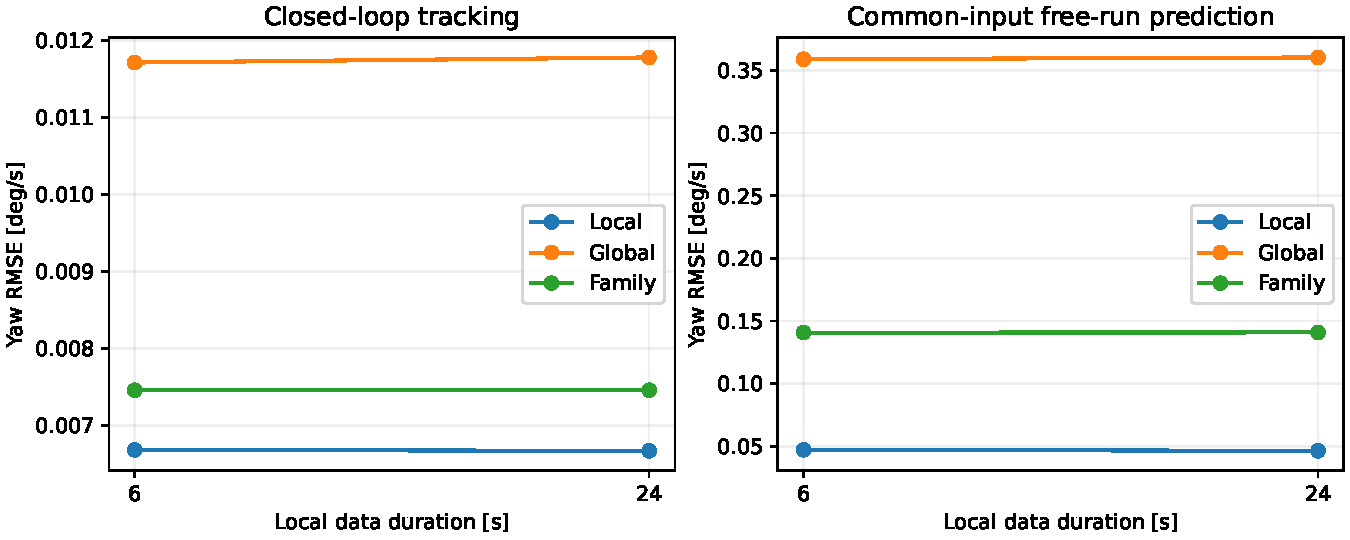
\includegraphics[width=\linewidth]{../results/figures/experiment_7a_local_identification.pdf}
\caption{Experiment 7A: noisy restricted-coverage results as local recording
duration increases. Closed-loop tracking and common-input prediction are
different evaluations; their absolute errors should not be equated.}
\label{fig:experiment7a}
\end{figure}

As shown in \cref{tab:experiment7a,fig:experiment7a}, family pooling increases
primary tracking error by 11.62\% relative to Local. The paired difference
$J_{\rm Local}-J_{\rm Family}$ is $-0.000776$ deg/s, with 95\% paired bootstrap
interval $[-0.000836,-0.000714]$ deg/s. None of the ten fleet pairs favors
Family. The predeclared collaboration gate therefore fails. Family pooling
does improve tracking by 36.33\% relative to Global, but this secondary
comparison cannot replace the failed Local comparison.

Local also has lower mean tracking error in all eight data conditions.
For short restricted records, removing measurement noise changes Local
tracking from 0.006681 to 0.006674 deg/s and its parameter error from 0.82\%
to 0.21\%. Extending noisy restricted records from six to 24 seconds lowers
Local parameter error to 0.41\%, but barely changes tracking (0.006669 deg/s).
Family tracking remains approximately 0.007457 deg/s. Thus local estimation
variance is already small in the tested regime. The physical three-ratio
structure permits generalization beyond a client's measured speed anchors;
restricted coverage does not by itself create a substantial information gap.
The persistence of the pooling penalty with clean and longer records supports
within-family approximation bias as the dominant explanation here. Nonlinear
model mismatch remains present, so this is evidence from controlled contrasts,
not an exact bias--variance decomposition.

The primary worst-family tracking errors are 0.006823, 0.007817, and 0.013517
deg/s for Local, Family, and Global, respectively. Steering RMS is approximately
0.80961 degrees for all three, with peak rates approximately 1.163 degrees/s.
The ordering is therefore not explained by a large steering-effort difference.
Family deploys three scheduled families instead of Local's 30, at an 11.62\%
relative tracking penalty (0.000776 deg/s absolute). This is a measurable
complexity--performance trade-off, not evidence that collaboration improves
individual prediction or tracking accuracy.

\paragraph{Consequence for the next experiment.}
Do not proceed to federated optimization with a claim that its accuracy benefit
has already been established. A useful next diagnostic is a predeclared
personalization comparison: local fitting, fixed oracle-family pooling, and
family-informed local regularization, with regularization chosen using training
validation only. This would test whether sharing can reduce uncertainty while
retaining client-specific differences. Any harder data regime must be motivated
independently and specified before testing, rather than increasing noise until
pooling wins. Learned clustering and decentralized optimization remain later
questions. The negative 7A gate is retained regardless of subsequent outcomes.

\paragraph{Reproducibility.}
The frozen protocol is \texttt{code/config/experiment\_7a.json}; the runner is
\texttt{code/experiments/experiment\_7a\_local\_identification.py}.
Per-seed compressed tables retain client metrics, fitted parameters, prediction
errors, and data manifests. Summary tables, paired comparisons, and the gate
decision are stored under \texttt{results/tables/experiment\_7a*}.
The \texttt{--summarize-only} option regenerates aggregate evidence without
refitting. Predictor integration, record resets, exact-parameter recovery,
and client-specific controller dispatch are covered by regression checks;
the complete suite contains 36 passing tests.
